\chapter{A Determinization Layer for Ludii}
\label{DeterminizationLayerLudii}

\begin{abstract}
The previous chapter demonstrated that native simulation-based agents in Ludii involuntarily access hidden game-state information through unrestricted context copies, producing artificially inflated performance figures in imperfect-information games. This chapter presents the solution developed in this thesis to address that problem.

The proposed approach introduces a determinization layer that intercepts simulation-time context copies, replaces hidden information with coherent hypotheses generated from past observations, and integrates transparently with any existing Ludii agent. The solution requires no modification to existing agent implementations and only a minimal, backward-compatible extension to the Ludii engine itself.

The chapter describes the architecture of the solution in full, covering hidden-information detection, game-history reconstruction, hypothesis generation, context injection, and agent integration.

The full implementation is available on \hyperlink{https://github.com/jejeAKAgg/TFE26-093}{GitHub}\footnote{\url{https://github.com/jejeAKAgg/TFE26-093}}, which includes the \LaTeX{} source for this thesis alongside the TAG and Ludii implementations as Git submodules.
\end{abstract}


%%% 5.1 %%%
\section{Design Principles and Overview}
\label{sec:solution_overview}

The core insight motivating the solution is straightforward: the problem identified in Chapter~\ref{HiddenInfoSimulationLudii} does not require replacing Ludii's simulation infrastructure. It only requires intercepting one specific operation, the context copy, and substituting a smarter version in its place.

Rather than letting \textsc{copyContext()} return a raw duplicate of the true game state, the determinization layer intercepts this call and returns a modified copy in which the opponent's hidden pieces have been replaced by a coherent hypothesis derived from the observations accumulated during gameplay. From the agent's perspective, the interface is identical: it receives a \textsc{Context} object and proceeds with its normal simulation logic. The difference lies entirely in what that context contains.

This design satisfies three requirements that shaped the architecture throughout its development. The solution must be \textbf{transparent to existing agents}: no modification to the internal decision logic of UCT, MAST, FlatMC, or any other Ludii agent should be necessary. It must be \textbf{generic across games}: the mechanism for detecting and replacing hidden information should work from the game's \textsc{.lud} description alone, without game-specific code. And it must be \textbf{minimally invasive with respect to Ludii's engine}: the framework should remain intact and backward-compatible, so that the solution does not break any existing perfect-information game or agent.

The solution is organized around three interdependent components. The \textbf{ContextDeterminiser} is responsible for analyzing the \textsc{.lud} file, reconstructing what the acting player can legitimately know at any point in the game, generating a coherent hypothesis for the hidden state, and injecting that hypothesis into a copy of the context before returning it. The \textbf{DeterminizationEngine} is the constraint-based hypothesis generator: a direct port of the engine developed in Chapter~\ref{BattleshipInTAG}, adapted to operate over Ludii's internal state representation rather than TAG's. The \textbf{DeterminizedAgent} is a lightweight wrapper that plugs the determinization layer into any existing Ludii agent by overriding the context copy mechanism, without touching the agent's decision logic.

These three components interact through a single integration point added to \textbf{AI.java}: a \textsc{setContextCopier()} method that allows an external component to replace the default copy strategy with a custom one. This is the only modification made to Ludii's core, and it is fully backward-compatible: agents that do not call \textsc{setContextCopier()} continue to use the standard raw copy, as before.

The design is closely related to the broader line of work on belief-state reasoning under hidden information~\cite{morenville2024beliefsg,morenville2025belief_constraints}. While those approaches focus on maintaining explicit probabilistic belief representations over game states, the present solution takes a determinization perspective: rather than tracking the full distribution, it samples plausible complete states consistent with past observations and uses them directly as simulation inputs. This tradeoff between representational completeness and computational tractability has been extensively studied in the imperfect-information search literature~\cite{cowling2012information}, and the choice here is deliberate: it allows the solution to remain computationally lightweight and directly compatible with standard MCTS-based agents.


%%% 5.2 %%%
\section{Detecting Hidden Information}
\label{sec:detect_hidden}

Before any hypothesis can be generated, the solution must determine what kind of hidden information the current game involves. This detection step is performed once at initialization by the \textbf{ContextDeterminiser}, which reads the raw content of the game's \textsc{.lud} file and identifies the \texttt{set Hidden} ludemes it contains.

As introduced in Chapter~\ref{Background}, Ludii encodes hidden information through three variants of this ludeme. The plain \texttt{(set Hidden ...)} form hides all chunk fields associated with a cell, including ownership, piece type, and state. The \texttt{(set Hidden Who ...)} variant hides only the ownership field, leaving the piece type visible, while \texttt{(set Hidden What ...)} hides only the piece type, leaving ownership exposed. By scanning the \textsc{.lud} file for these patterns, the \textbf{ContextDeterminiser} determines which fields need to be replaced during the context copy.

Three internal hidden-type categories are defined accordingly. When ownership is hidden, the agent does not know which cells are occupied by opponent pieces: this is the \texttt{WHO} category, which corresponds to Battleship, where the entire enemy fleet is invisible. When piece type is hidden but location is visible, the agent knows where pieces are but not what they are: this is the \texttt{WHAT} category, corresponding to games like Stratego. When both are hidden simultaneously, the \texttt{WHO\_AND\_WHAT} category applies, as in card games where neither the presence nor the identity of opponent cards is known.

For Battleship, the \textsc{.lud} file uses the plain \texttt{(set Hidden ...)} form without suffix, which the \textbf{ContextDeterminiser} maps to \texttt{WHO\_AND\_WHAT} by default. In practice, since the engine generates spatial presence hypotheses rather than type hypotheses, only the \texttt{who} chunk field is replaced in the injected copy. Extending the engine to also reconstruct \texttt{what} values, for games like Stratego, is a natural direction for future work.


%%% 5.3 %%%
\section{Reconstructing the Game History}
\label{sec:history_reconstruction}

Generating a coherent hypothesis requires knowing what the acting player has legitimately observed so far. In TAG, this information is maintained explicitly in the game state: the \texttt{player0ShotGrid} and \texttt{player1ShotGrid} structures record every hit and miss as they occur. In Ludii, the equivalent information must be reconstructed from the game's \textsc{Trial} object, which records the full sequence of actions applied since the start of the game.

The \textbf{ContextDeterminiser} iterates over the move history stored in the \textsc{Trial}, filtering for actions that correspond to shots fired by the acting player and their outcomes. For each such action, it recovers the target cell and the result: a hit if the action modified the state of a hidden cell, a miss otherwise. This reconstruction produces the same two structures that the TAG engine relies upon: a \textit{hitMap}, recording confirmed occupied cells, and a \textit{missMap}, recording confirmed empty cells.

The reconstruction is performed fresh at each copy call rather than maintained incrementally. This is intentional: it avoids any need to track state between calls and ensures that the maps always reflect the complete history available in the \textsc{Trial} at the time of the simulation. The computational overhead is proportional to the number of moves played, which in Battleship is at most 100 per player and therefore negligible relative to the cost of hypothesis generation itself.

One subtlety arises with the sinking of ships. In standard Battleship, when a ship is completely sunk, the opponent is informed of both the sink event and the ship's size. This information further constrains the set of valid configurations: the \textbf{ContextDeterminiser} incorporates sink events from the history to mark entire ship footprints as confirmed occupied, reducing the search space for subsequent hypothesis generation.


%%% 5.4 %%%
\section{The Determinization Engine}
\label{sec:det_engine}

The \textbf{DeterminizationEngine} is the core computational component of the solution. Its role is to produce a plausible complete hidden-state configuration, consistent with all observations reconstructed from the game history, that can be injected into the context copy before it is returned to the agent.

The engine is a direct port of the Constraint-Based Determinization developed in Chapter~\ref{BattleshipInTAG}, adapted to operate over Ludii's internal \textsc{Context} representation rather than TAG's \textsc{AbstractGameState}. The constraint satisfaction logic, the placement algorithm, and the fallback behavior are identical to those described in Section~3.3 and Section~3.4.2. Ships are placed sequentially while respecting the \textit{missMap} as a set of forbidden cells and the \textit{hitMap} as a set of cells that must be covered. When multiple valid placements exist, the engine samples among them to preserve diversity across simulations. When no valid configuration can be found within the allotted attempts, the engine falls back to unconstrained random placement, ensuring termination under all circumstances.

The only adaptation required concerns how cell values are read and written. In TAG, the hypothesis is written into a \textsc{GridBoard} object. In Ludii, the engine writes directly into the \textsc{State} substructure of the copied \textsc{Context}, setting the \texttt{who} chunk field of each cell to reflect the generated hypothesis. Cells belonging to the opponent's hidden region that are not occupied in the hypothesis have their \texttt{who} field set to zero; cells covered by a hypothesized ship have their \texttt{who} field set to the opponent's player index. All other fields, including the \texttt{what} and \texttt{state} values for non-hidden cells, are left untouched.

This targeted field-level modification ensures that the rest of the \textsc{Context} remains intact and consistent. The legal move generator, the rule interpreter, and all other engine components continue to operate on a valid game state; only the hidden region has been replaced with a hypothesis.


%%% 5.5 %%%
\section{Injecting the Hypothesis}
\label{sec:injection}

Once the \textbf{DeterminizationEngine} has produced a valid hypothesis, the \textbf{ContextDeterminiser} injects it into the context copy before returning it to the calling agent. The injection procedure operates as follows.

A standard \textsc{copyContext()} call is first made to obtain a faithful structural copy of the current game state. This copy is then passed to the engine, which identifies the cells belonging to the opponent's hidden region using the \texttt{set Hidden} information extracted during the detection step, and overwrites their \texttt{who} fields with the values dictated by the generated hypothesis.

The result is a \textsc{Context} object that is identical to the true game state in all observable aspects, but whose hidden region reflects a plausible fictional world consistent with the acting player's observations rather than the true ship layout. This context is then returned to the calling agent in place of the raw copy it would have received from the standard \textsc{copyContext()} mechanism.

The injection is entirely transparent to the agent. From its perspective, it called a copy method and received a \textsc{Context} object. Whether that object reflects the true state or a coherent hypothesis is not visible to the agent, nor does it need to be: the agent simply runs its simulation on the provided context and uses the result to evaluate candidate actions.


%%% 5.6 %%%
\section{The DeterminizedAgent}
\label{sec:determinized_agent}

The final component of the solution is the \textbf{DeterminizedAgent}, a generic wrapper that integrates the determinization layer into any existing Ludii agent without modifying that agent's source code.

The wrapper extends \textbf{AI.java} and holds a reference to an inner agent, which can be any standard Ludii agent such as UCT, MAST, or FlatMC. At initialization, the \textbf{DeterminizedAgent} instantiates a \textbf{ContextDeterminiser} for the current game, which performs the hidden-information detection described in Section~\ref{sec:detect_hidden}. It then calls \textsc{setContextCopier()} on the inner agent, providing the \textbf{ContextDeterminiser} as the custom copy strategy. From this point forward, every time the inner agent calls \textsc{copyContext()} during search, the call is routed through the \textbf{ContextDeterminiser} instead of the standard engine copy, and the agent receives determinized contexts rather than raw ones.

The decision logic of the inner agent is completely untouched. UCT still builds its search tree using UCB1 selection; MAST still maintains move-average statistics; FlatMC still evaluates actions through flat Monte Carlo rollouts. The only change is the quality of the context those algorithms receive: rather than reasoning about the true hidden state, they reason about coherent hypothetical worlds derived from what they have observed.

This architecture has an important practical implication: the determinization layer can be applied retroactively to any existing Ludii agent. No game-specific knowledge, no modification of the agent's decision logic, and no recompilation of the original agent are required. The \textbf{DeterminizedAgent} wrapper and the single \textsc{setContextCopier()} method added to \textbf{AI.java} are the only additions needed to equip the entire existing Ludii agent ecosystem with coherent hidden-information reasoning.

Figure~\ref{fig:determinization_pipeline} provides an overview of the complete pipeline, from the moment an agent requests a context copy to the moment it receives the determinized result.

\begin{figure}[H]
    \centering
    % TODO: Insert pipeline diagram here (ContextDeterminiser flow:
    % agent calls copyContext -> intercepted by DeterminizedAgent ->
    % ContextDeterminiser reconstructs history -> DeterminizationEngine
    % generates hypothesis -> hypothesis injected into copy ->
    % determinized Context returned to agent)
    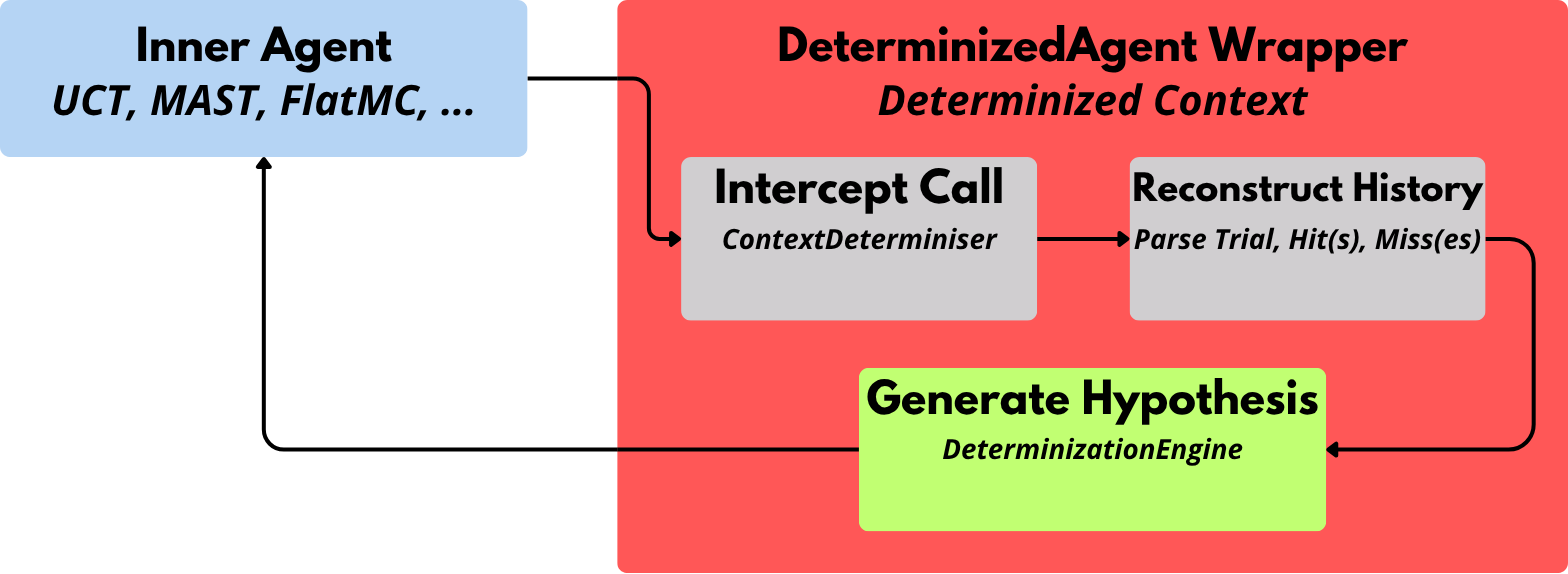
\includegraphics[width=\textwidth]{figs/background/determinization_pipeline.png}
    \captionsetup{justification=centering}
    \caption{The determinization pipeline. When the inner agent requests a context copy, the \textbf{DeterminizedAgent} intercepts the call, reconstructs the game history from the \textsc{Trial}, generates a coherent hidden-state hypothesis, injects it into the copy, and returns the modified context to the agent.}
    \label{fig:determinization_pipeline}
\end{figure}


%%% 5.7 %%%
\section{Discussion and Limitations}
\label{sec:solution_discussion}

The solution achieves its three design requirements. It is transparent to existing agents, generic with respect to the game description, and minimally invasive with respect to Ludii's engine. The \textsc{setContextCopier()} extension to \textbf{AI.java} is the only structural change made to the framework, and it is fully backward-compatible.

Several limitations are worth acknowledging. The current implementation handles only the \texttt{who} chunk field, addressing hidden-position games such as Battleship. Games involving hidden piece identities, such as Stratego, would require the engine to also generate hypotheses for \texttt{what} values, which in turn requires reasoning about type constraints rather than purely positional ones. This extension is conceptually straightforward but was left outside the scope of the present work.

History reconstruction from the \textsc{Trial} relies on the assumption that all relevant observations can be inferred from the move sequence alone. This holds for Battleship, where every shot has a deterministic and immediately observable outcome. In games with more complex information structures, such as simultaneous moves, hidden draws, or probabilistic events, the reconstruction may require access to additional game-specific signals not encoded in the standard move history.

Finally, the determinization approach adopted here inherits the known limitations of single-determinization search. As discussed in the context of Chapter~\ref{BattleshipInTAG}, the quality of the agent's decisions is bounded by the quality of the hypotheses it reasons about. Approaches that maintain richer uncertainty representations, such as the belief-state models\cite{morenville2025belief_constraints,morenville2024beliefsg}, can in principle reason more accurately under uncertainty, at the cost of substantially greater computational complexity. The present solution prioritizes tractability and generality over representational completeness, which appears well-suited to the GGP setting where agents must operate across many different games without game-specific tuning.
